\chapter{Measurement Setup and Evaluation}
\newcommand{\rd}[1]{\textcolor{red}{#1}}
\newcommand{\gn}[1]{\textcolor{green}{#1}}

\label{Chapter5}

%To evaluate my improvements i will first describe the test beds and data sets used for the evaluation. I will then talk about the experiment performed on the individual components, room recognition and weighting, and then present the final evaluation of the entire system.

In this chapter I will evaluate the system. First I will present the results of the two experiments and then I will evaluate the complete system.

\section{Experiment: Room Recognition}
The goal of this experiment, is to evaluate the performance of different fingerprinting maps and to test the feasibility of this proposed room recognition system.

The objective was to answer the following questions:
\begin{itemize}
\item \red{What is the best way to gather the RPs for the fingerprinting-map How many RPs are needed and how does their distribution affect the accuracy?}
\item How does the magnetic field data influence the accuracy. Does it improve the accuracy as presumed?
\item What accuracy can be expected form the system. Does it even achieve high enough accuracy?
\end{itemize}

\subsection{Setup}
For this the four data sets from the apartment test bed were combined to generate fingerprinting maps with different characteristics. \red{The performance of these maps was determined by training a SVM classifier with the map and testing the classifier on the remaining data-sets not used for the map.}

This was done both with and without using magnetic field data, in order to evaluate the impact \red{of magnetic field data} on the performance.

\subsection{Results}
The table below shows the performance of the different fingerprinting maps. The fist row details the training data and the following rows the accuracy for a given test set, fist without and then with magnetic field data.

\begin{table}
\label{tab:AccuracyRoomRecognitionExperiment}
\centering
\begin{tabular}{l l l l l}
\toprule
\tabhead{Training Data (\#Samples)} & \multicolumn{4}{c}{\tabhead{Testing Data (w/o \(B\)|w/ \(B\))}} \\
 & LD & HD & B & C\\
\midrule
LD (42) & - & 78.5\%|\rd{-1.1\%} & 55.2\%|\gn{6\%}& 100\%|0\%\\
HD (186) & 88.0\%|\rd{-9.43\%}& - & 73.1\%|\gn{3\%}& 100\%|0\%\\
B (67) & 83.3\%|\rd{-16.6\%}& 81.7\%|\rd{-0.6\%}& - & 91.3\%|\gn{4.3\%}\\
B+C (90) & 85.7\%|\rd{-2.2\%}& 88.7\%|\rd{-3.2\%}& - & -\\
B+LD (109) & - & 84.9\%|\gn{0.6\%}& - & 95.7\%|\gn{4.3\%}\\
\bottomrule
\end{tabular}
\caption{Performance of the room recognition with different fingerprinting maps with 7 AN}
\end{table}

\begin{table}
\label{tab:AccuracyRoomRecognition}
\centering
\begin{tabular}{l l l l l}
\toprule
\tabhead{Training Data (\#Samples)} & \multicolumn{4}{c}{\tabhead{Testing Data (w/o \(B\)|w/ \(B\))}} \\
 & LD & HD & B & C\\
\midrule
LD (42) & - & 69.4\%|\rd{-2.8\%} & 50.7\%|\gn{3.3\%}& 87.0\%|0\%\\
HD (186) & 78.6\%|\rd{-11.9\%}& - & 47.8\%|\gn{7.42\%} & 78.3\%|\gn{8.7\%} \\
B (67) & 57.1\%|\rd{-7.1\%} & 58.6\%|\gn{0.5\%} & - & 56.52\%|\rd{-13.02\%}\\
B+C (90) & 61.9\%|\gn{9.5\%} & 57.0\%|\gn{9.1\%}& - & -\\
B+LD (109) & - & 76.9\%|\rd{-7\%} & - & 82.6\%|\gn{4.4\%}\\
\bottomrule
\end{tabular}
\caption{Performance of the room recognition with different fingerprinting maps with 4 AN}
\end{table}

Magnetic field performance measurements yielded the following results:

\begin{table}
\label{tab:Ex1MagneticField}
\centering
\begin{tabular}{l l l}
\toprule
\tabhead{Average with MF} & \tabhead{Average without MF} & \tabhead{T-Test tobs} \\
\midrule
88.561625\% & 87.899235\% & 1 \\
\bottomrule
\end{tabular}
\caption{Averages of 20 runs and the T-Test results}
\end{table}

The theoretical limit with a student's distribution and 19 degrees of freedom with a confidence level of 5\% is  2.093. The difference between the two sets of samples is not statistically significant.


\subsection{Discussion}

The two main conclusions from this experiment are:

\red{the best way to gather the maps is}

\red{magnetic feld data is important}

Furthermore this shows that simple room recognition can be achieved by easily and in residential eras with numerous wifi signals id doesn't even need additional infrastructure.


\section{Experiment: Weighting}
In this experiment different weighting models are compared in order to answer the question from section \ref{WeightingModelDefinition}.

\subsection{Setup}
The models, both ranging and weighting, are trained with the entire \emph{Ranging data} set from the IAM-Building test bed. For evaluation the same data-set is used with the assumption of 100\% room recognition accuracy.

The following models were compared:

\begin{itemize}
\item Room Weights
\item Room + distance weights
\item Room + distance weights with thresholds

\note{insert description of models here}
\end{itemize}

\subsection{Results}
One way to visualize the performance of localization systems is to plot the cumulative distribution function of the localization error. This allows for a more accurate representation of the performance than just using statistical values like the mean and standard deviation.

The performance if the weighting models is compared to distance based weights from the existing approach and weights using no weights at all (OLS).

\begin{figure}[htp]

\label{fig:SVM}
\centering
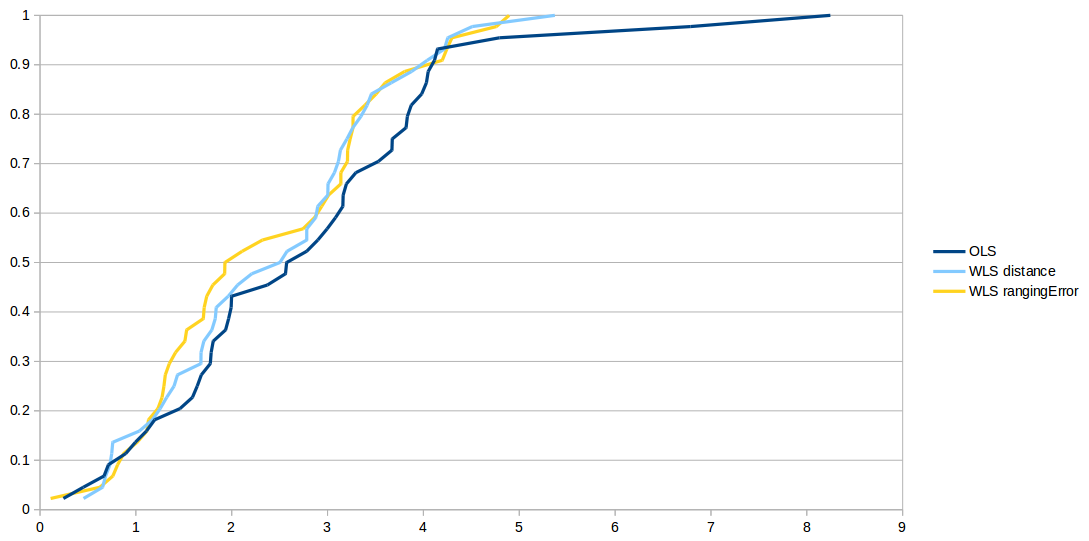
\includegraphics[width=\textwidth]{Figures/Weighting1.png}
\decoRule
\caption[...]{...}

\end{figure}
\begin{figure}[htp]

\label{fig:SVM}
\centering
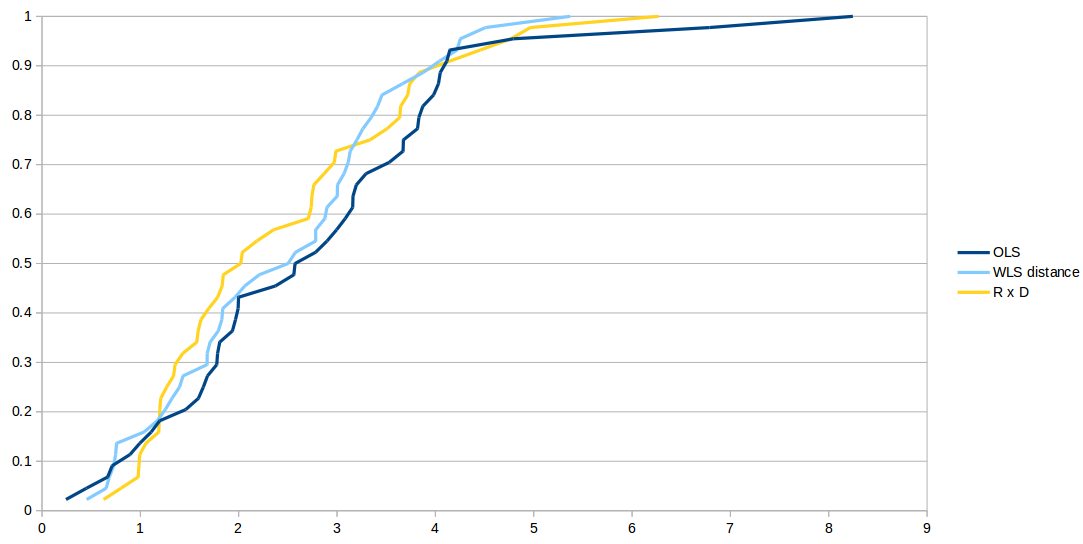
\includegraphics[width=\textwidth]{Figures/Weighting2.png}
\decoRule
\caption[...]{...}

\end{figure}
\begin{figure}[htp]

\label{fig:SVM}
\centering
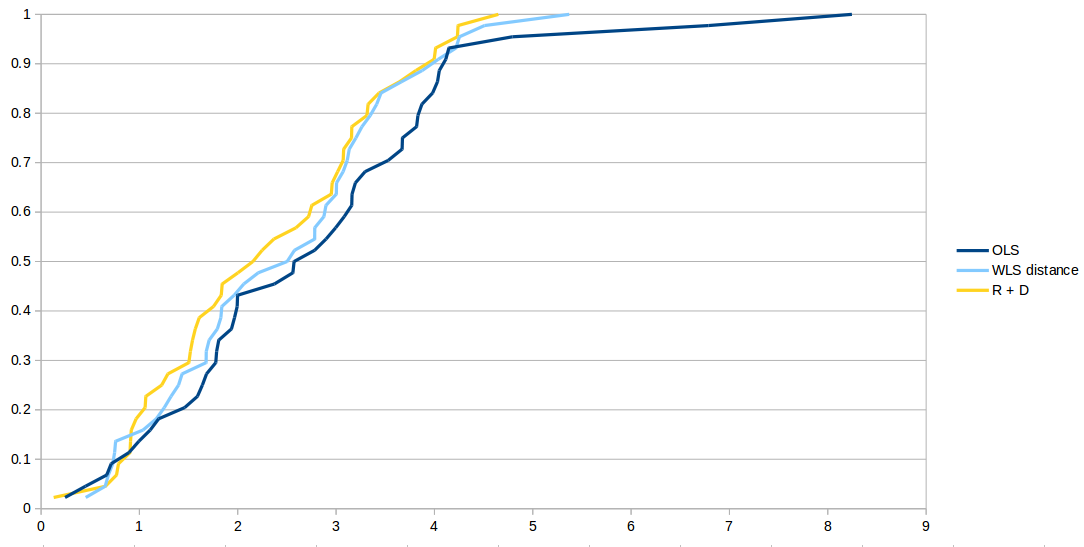
\includegraphics[width=\textwidth]{Figures/Weighting3.png}
\decoRule
\caption[...]{...}

\end{figure}
\begin{figure}[htp]

\label{fig:SVM}
\centering
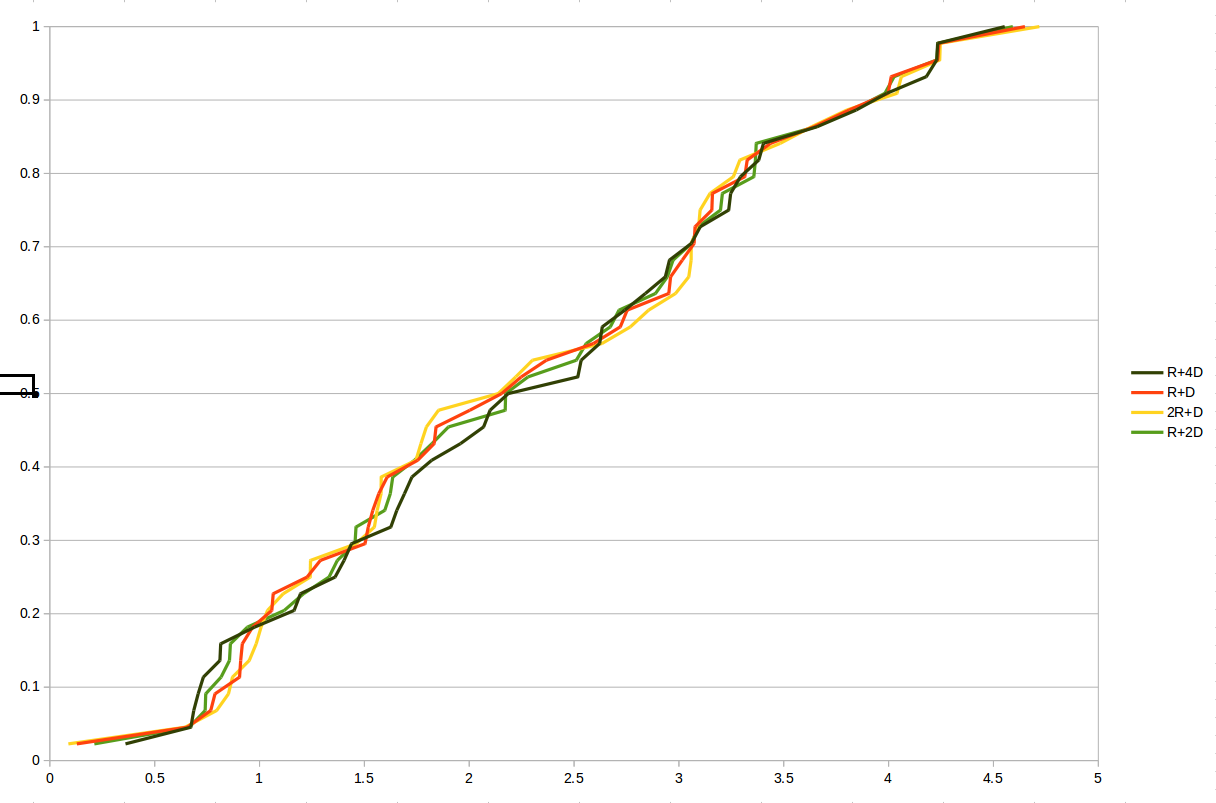
\includegraphics[width=\textwidth]{Figures/Weighting4.png}
\decoRule
\caption[...]{...}

\end{figure}

\paragraph{Discussion}

\section{Final Evaluation}

To evaluate the compete system I used the process described in section \ref{technicalImplementation}. The entire \emph{Ranging data} set was used for training and testing.

\subsection{Setup}
In a first step the room recognition is evaluated with two different testing data-sets. Then the localization error of the complete system is determined using the \emph{Ranging data} set for testing.

\subsection{Results}

\begin{figure}[htp]

\label{fig:SVM}
\centering
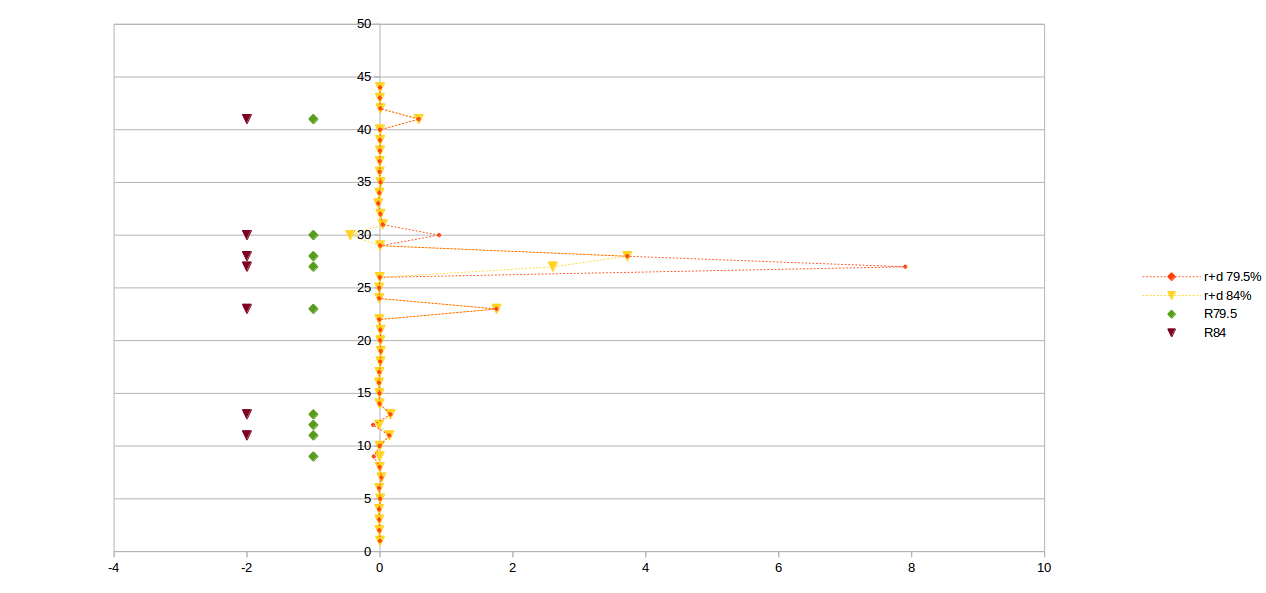
\includegraphics[width=\textwidth]{Figures/Difference1.png}
\decoRule
\caption[...]{...}

\end{figure}
\begin{figure}[htp]

\label{fig:SVM}
\centering
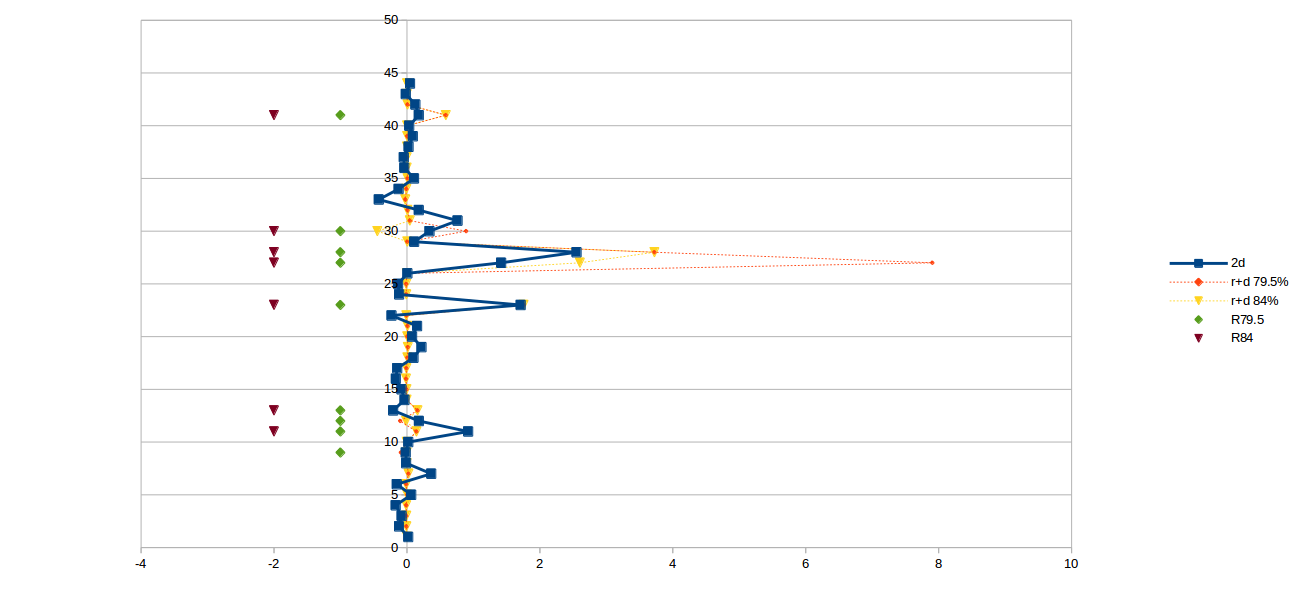
\includegraphics[width=\textwidth]{Figures/Difference2.png}
\decoRule
\caption[...]{...}

\end{figure}
\begin{figure}[htp]

\label{fig:SVM}
\centering
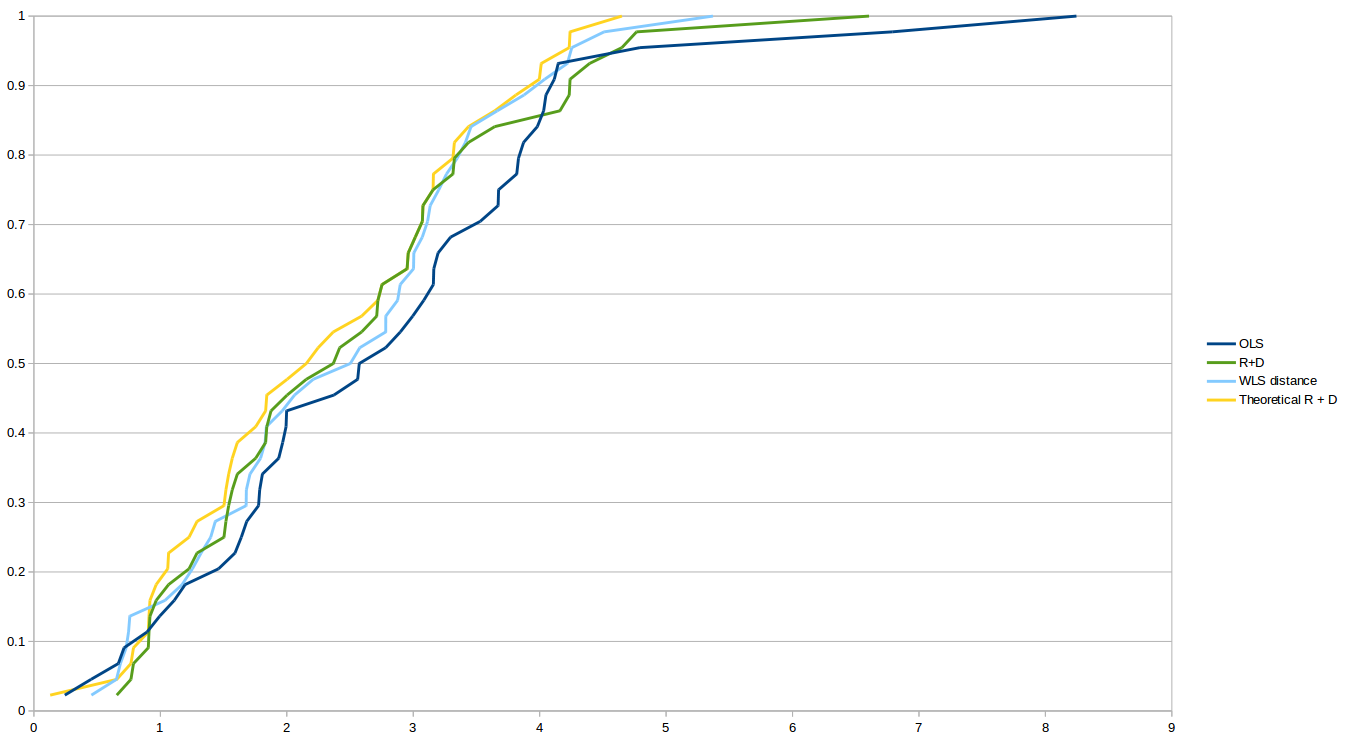
\includegraphics[width=\textwidth]{Figures/final.png}
\decoRule
\caption[...]{...}

\end{figure}
